\documentclass[../../main/main.tex]{subfiles}
\graphicspath{{./figures/}}

\dominitoc
\faketableofcontents

\makeatletter
\renewcommand{\@chapapp}{Chimie -- chapitre}
\makeatother

% \toggletrue{student}
% \HideSolutionstrue
\toggletrue{corrige}
\renewcommand{\mycol}{black}
% \renewcommand{\mycol}{gray}

\begin{document}
\setcounter{chapter}{0}

\chapter{Introduction \`a la chimie}

\vfill

\begin{prgm}
	\begin{tcb}*(ror)"know"{Savoirs}
		\begin{itemize}[label=$\diamond$, leftmargin=10pt]
			\item Recenser les espèces physico-chimiques présentes
			      dans un système.
			\item Décrire la composition d’un système à l’aide des grandeurs physiques
			      pertinentes.
			\item Identifier le caractère extensif ou intensif d’une
			      variable.
		\end{itemize}
	\end{tcb}

	\begin{tcb}*(ror)"how"{Savoir-faire}
		\begin{itemize}[label=$\diamond$, leftmargin=10pt]
			\item Écrire l’équation de la réaction (ou des réactions) qui modélise(nt)
			      une transformation chimique donnée.
		\end{itemize}
	\end{tcb}
\end{prgm}

\vfill
\minitoc
\vfill

\newpage

La chimie se concentre à décrire la matière et ses transformations, mais
lesquelles~? Comment caractérise-t-on physiquement et mathématiquement les états
et leurs transformations~?

\section{Vocabulaire général}
\subsection{Atomes et molécules}

\subsubsection{Les atomes}
L'atome est un constituant \textbf{neutre} de la matière, comportant un
noyau central entouré d'un nuage électronique. Le noyau est composé de
particules nommées \textbf{nucléons} dont il existe deux sortes~:
\begin{itemize}
	\bitem{les protons}, de charge $+e$ et de masse $m_p =
		\csw{\SI{1.673e-27}{kg}}$~;
	\bitem{les neutrons}, de charge nulle et de masse $m_n =
		\csw{\SI{1.675e-27}{kg}}$.
\end{itemize}
La taille du noyau d'un atome est de l'ordre de \SI{e-15}{m}, soit
\SI{1}{fm} (femtomètre).
\smallbreak
Le nuage électronique est composé
\begin{itemize}
	\item d'\textbf{électrons}, de charge $-e$ et de masse $m_e =
		      \csw{\SI{9.1e-31}{kg}}$.
\end{itemize}
Un atome avec son nuage électronique fait une taille de l'ordre de
\SI{e-10}{m} soit \SI{0.1}{nm}.

\begin{tcb}[label=def:numéroatomique,
		sidebyside, righthand ratio=.2](defi){Numéro atomique et nombre de nucléons}
	Pour représenter un atome de façon symbolique, on utilise son symbole
	chimique, noté X ici dans le cas général, accompagné de deux nombres~:
	\begin{itemize}
		\item \csw{
			      Son \textbf{numéro atomique}, soit le nombre de \textbf{protons}
			      contenus dans le noyau. Il est noté $Z$, et définit l'élément
			      chimique~;
		      }
		\item \csw{
			      Le \textbf{nombre de nucléons}, également appelé le \textbf{nombre
				      de masse}, noté $A$.
		      }
	\end{itemize}
	\tcblower
	On écrit alors
	\csw{
		\[
			\ce{^{A}_{Z}X}
		\]
	}
\end{tcb}

\begin{tcb}[label=rema:atomeneutre](rema){Nombre d'électrons et de masse}
	Un atome étant neutre, indiquer son nombre de protons suffit~: le nuage
	électronique sera constitué d'autant d'électrons que de protons dans le
	noyau.
	\smallbreak
	De plus, les électrons étant $\approx 1000$ fois plus légers que les
	nucléons, on les néglige souvent dans le calcul de la masse d'un atome, d'où
	l'appellation \textbf{nombre de masse} pour $A$.
\end{tcb}
\begin{tcb}[label=exem:atomes](appl){Application}
	Donner la composition des atomes suivants~:
	\smallbreak
	\begin{isd}
		\begin{itemize}
			\item L'atome de bore \ce{^{10}_{5}B}
			      \smallbreak
			      \csw{5 protons, et $10-5=5$ neutrons}
			\item L'atome d'oxygène $\ce{^{16}_{8}O}$
			      \smallbreak
			      \csw{8 protons et $16-8=8$ neutrons~;}
		\end{itemize}
		\tcblower
		\begin{itemize}
			\item L'atome de fer $ \ce{^{56}_{26}Fe}$
			      \smallbreak
			      \csw{26 protons et $56-26 = 30$ neutrons;}
			\item L'atome de plomb $\ce{^{208}_{82}Pb}$
			      \smallbreak
			      \csw{82 protons et $208 - 82 = 126$ neutrons.}
		\end{itemize}
	\end{isd}
\end{tcb}

\subsubsection{Les ions}

\begin{tcb}[label=def:ion](defi){Ion}
	Un \textbf{ion} est un atome qui a \textbf{perdu ou gagné un ou plusieurs
		électrons}. On indique leur charge en haut à droite de l'élément chimique.
	On a alors deux types d'ions~:
	\begin{itemize}
		\item \csw{
			      les \textbf{cations} qui sont chargés \textbf{positivement},
			      c'est-à-dire que c'est un atome qui a \textbf{perdu} un ou plusieurs
			      électrons~;
		      }
		\item \csw{
			      les \textbf{anions} qui sont chargés \textbf{négativement},
			      c'est-à-dire que c'est un atome qui a \textbf{gagné} un ou plusieurs
			      électrons.
		      }
	\end{itemize}
\end{tcb}
\begin{tcb}[label=exem:ion](appl){Application}
	Donner le nombre de protons et d'électrons des ions suivants~:
	\smallbreak
	\begin{isd}
		\begin{itemize}
			\item L'ion sodium \ce{_{11}Na^{+}}
			      \smallbreak
			      \csw{11 protons, et donc 10 électrons.}
			\item L'ion chlorure \ce{_{17}Cl^{-}}
			      \smallbreak
			      \csw{17 protons et donc 18 électrons.}
		\end{itemize}
		\tcblower
		\begin{itemize}
			\item L'ion fer \ce{_{26}Fe^{2+}}
			      \smallbreak
			      \csw{26 protons, 24 électrons.}
			\item L'ion oxyde \ce{_{16}O^{2-}}
			      \smallbreak
			      \csw{16 protons et 18 électrons.}
		\end{itemize}
	\end{isd}
\end{tcb}

\subsubsection{Les molécules}
\begin{tcb}[label=def:molécules](defi){Molécules}
	Les molécules ou les ions polyatomiques sont des assemblages d'atomes
	liés entre eux grâce à des liaisons chimiques. Ces liaisons chimiques se
	créent dès que l'énergie des atomes «~liés~» est plus faible que la
	somme des énergies des atomes séparés.
	\smallbreak
	Ainsi, des atomes engagés dans une molécule sont \textbf{plus stables} que
	s'ils étaient seuls, d'où l'existence des molécules.
\end{tcb}
\begin{tcb}[label=exem:molécules](exem){Molécules}
	\begin{itemize}
		\item Le méthane est l'assemblage d'un atome de carbone et de 4
		      atomes d'hydrogène~: on l'écrit CH$_4$~;
		\item Le dioxygène est la molécule composée de deux atomes d'oxygène
		      liés entre eux~: on l'écrit O$_2$.
	\end{itemize}
\end{tcb}

\subsection{Classification par composition}

\begin{center}
	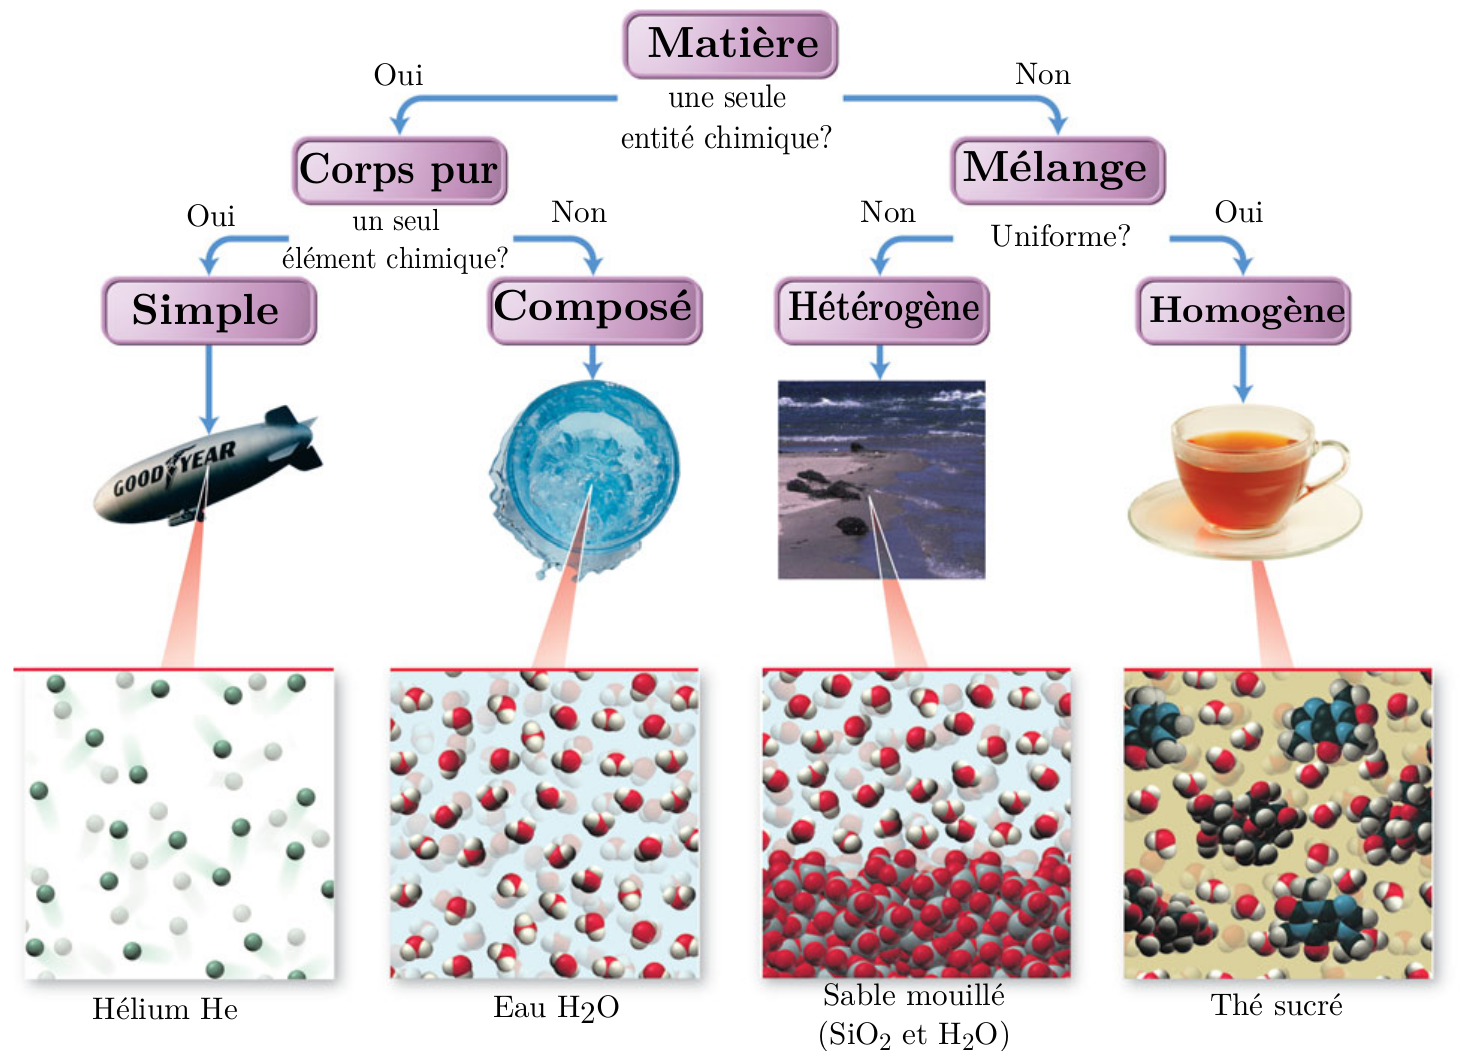
\includegraphics[width=.95\linewidth]{compo}
\end{center}

\subsection{États de la matière}
\begin{tcb}[label=def:etat, sidebyside, sidebyside align=top,
		righthand ratio=.6](defi)
	{États ou phases de la matière}
	\tcbsubtitle{\fatbox{Définition d'une phase}}
	\csw{
		Zone de l'espace où les grandeurs physiques locales (pression, température,
		…) varient de manière continue. Lorsque le corps évolue d’une phase à
		l'autre, on parle de \textbf{transition de phase}.
	}
	\tcbsubtitle{\fatbox{Phase ordonnée ou non}}
	\begin{itemize}
		\bitem{Désordonnée}~: \csw{
			les entités la composant peuvent bouger les unes par rapport aux autres
		}
		\bitem{Ordonnée}~: \csw{
			les entités sont fixes les unes par rapport aux autres.
		}
	\end{itemize}
	\tcblower
	\tcbsubtitle{\fatbox{Différentes phases}}
	\begin{itemize}
		\bitem{Solide}~: \csw{
			un solide a une forme propre, un volume propre, et peut être ordonné
			(cristal) ou non (verre)~;
		}
		\vspace{-15pt}
		\bitem{Liquide}~: \csw{
			un liquide est dense mais désordonné, et prend la forme de son contenant~;
		}
		\bitem{Gazeux}~: \csw{
			un gaz est très peu dense et désordonné, et occupe \textit{tout le volume
				acessible}~;
		}
	\end{itemize}
	\begin{center}
		\switch{
			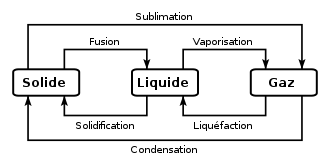
\includegraphics[width=.8\linewidth, draft=true]{trans_phase}
		}{
			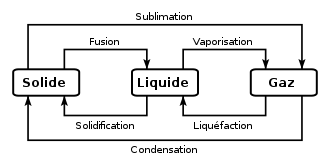
\includegraphics[width=.8\linewidth]{trans_phase}
		}
		\captionof{figure}{Vocabulaire transitions de phase}
	\end{center}
\end{tcb}

\begin{tcb}[label=def:solu](defi){Solutés et solutions}
	\begin{itemize}
		\bitem{Solution}~: \csw{
			résultat de la dissolution d'un composé chimique dans un liquide nommé
			\textbf{solvant}.
		}
		\bitem{Soluté}~: \csw{
			espèce chimique en solution.
		}
		\bitem{Solution aqueuse}~: \csw{
			soluion dont le solvant est l'eau
		}
	\end{itemize}
	Avant dissolution, l'espèce en question peut être un solide, un liquide
	ou un gaz. Elle peut être constituée d'ions ou de molécules.
\end{tcb}
\begin{tcb}[label=exem:solution](exem){Solutions}
	On peut dissoudre~:
	\begin{itemize}
		\item De l'acide chlorhydrique gazeux dans de l'eau~;
		\item De l'éthanol liquide dans de l'eau~;
		\item Du sel (NaCl, solide ionique) dans de l'eau (les ions Na$^+$ et
		      Cl$^-$ sont alors dissociés)~;
		\item Du sucre (solide moléculaire) dans de l'eau~;
		\item Du diiode dans de l'acétone…
	\end{itemize}
\end{tcb}

\begin{tcbraster}[raster columns=2, raster equal height=rows]
	\begin{tcb}[label=nota:état](nota){État de la matière}
		Les états des composés chimiques sont indiqués généralement en indice et
		toujours entre parenthèses. On note~:
		\begin{itemize}
			\item (g) pour un gaz~;
			\item (liq) ou (l) pour un liquide~;
			\item (s) pour un solide~;
			\item (aq) pour un soluté.
		\end{itemize}
	\end{tcb}
	\begin{tcb}[label=exem:notationétat](exem)'r'{Notations}
		\begin{itemize}
			\item Par exemple $\ce{O2\gaz{}}$~;
			\item Par exemple $\ce{H2O}_{\rm (liq)}$~;
			\item Par exemple $\ce{Fe\sol{}}$~;
			\item Par exemple $\ce{Na+\aqu{}}$.
		\end{itemize}
		La dissolution du sel $\ce{NaCl}\sol$ dans l'eau donne une solution composée
		d'eau liquide $\ce{H2O}\liq$, d'ion sodium $\ce{Na+}\aqu$ et d'ion chlorure
		$\ce{Cl-}\aqu$.
	\end{tcb}
\end{tcbraster}

\subsection{Systèmes physico-chimiques}
\begin{tcb}[label=def:système, tabularx={Y|Y|Y}](defi){Systèmes}
	\textbf{Système} & \textbf{Fermé} & \textbf{Isolé}
	\\\hline
	\csw{
		Ensemble de substances incluses dans une zone de l'espace \textbf{délimitée
			par une surface fermée} (réelle ou fictive), appelée surface frontière.
	}
	&
	\csw{
		N'échange pas de \textbf{matière} avec le milieu extérieur. Dans la suite du
		cours, on ne considérera que des systèmes fermés.
	}
	&
	\csw{
		N'échange ni \textbf{matière} ni \textbf{énergie} avec l'extérieur.
	}
\end{tcb}

\subsection{Transformations de la matière}

La matière peut subir des transformations de différentes natures, qui sont
traduites par des \textbf{équations-bilan}, qui indique~:
\begin{itemize}
	\item \csw{
		      les éléments de départ (\textbf{réactifs}) et les éléments de fin
		      (\textbf{produits})~;
	      }
	\item \csw{
		      les phases de chaque constituant~;
	      }
	\item \csw{
		      les proportions dans lesquelles ils apparaissent.
	      }
\end{itemize}

\begin{tcb}(defi){Nombres stœchiométriques}
	Les coefficients devant les espèces sont appelés \textbf{nombres
		stœchiométriques}. Ils sont généralement entiers pour représenter la réalité
	physico-chimique d'une réaction, mais peuvent être fractionnaires par
	simplicité mathématique.
\end{tcb}


Le signe entre les réactifs et produits
peut être une flèche simple de gauche à droite ou de droite à gauche,
les deux flèches ensemble ou un signe égal, selon les propriétés de la
réaction~:
\begin{itemize}
	\item $\ce{=}$ quand on fait un bilan de matière sans supposer le sens réel de
	      la réaction~;
	\item $\ce{->}$ pour indiquer que la réaction ne peut se faire dans l'autre
	      sens~;
	\item $\ce{<=>}$ si les deux sens sont possibles et s'équilibrent
\end{itemize}
Ces notions précises font l'objet des chapitres suivants.

\begin{tcb}(exem){Exemples}
	\vspace{-15pt}
	\begin{align*}
		\ce{Reactifs          & -> Produits
		\\
		aA + bB               & <=> cC + dD
		\\
		CH4\gaz{} + 2O2\gaz{} & = CO2\gaz{} + 2H2O\gaz{}
		}
	\end{align*}
\end{tcb}

\begin{tcb}[label=rema:eqbil](ror){Équation bilan}
	\begin{itemize}
		\item L'équation-bilan ne fait apparaître \textbf{que les espèces qui se
			      transforment}\ftn{Il est possible de faire apparaître les
			      espèces nécessaires à la réaction au-dessus de la flèche.}~;
		\item Après l'écriture d'une réaction, il faut \textbf{toujours}
		      vérifier qu'elle est équilibrée, tant en \textbf{nombre d'atome}
		      qu'en \textbf{nombre de charges}.
	\end{itemize}
\end{tcb}

\subsubsection{Transformations nucléaires}

\begin{tcbraster}[raster columns=2, raster equal height=rows]
	\begin{tcb}[label=def:transnuc](defi){Transformations nucléaires}
		\csw{
			Au cours d'une \textbf{transformation nucléaire}, un ou plusieurs
			\textbf{noyaux} atomiques sont modifiés.
		}
	\end{tcb}
	\begin{tcb}[label=exem:transnuc](exem)'r'{Transformation nucléaire}
		Lors de la désintégration radioactive (type $\alpha$) de l'uranium 238,
		le noyau d'uranium perd 4 nucléons, 2 protons et 2 neutrons.
		\csw{
		\[
			\ce{^{238}_{92}U}
			\longrightarrow
			\ce{^{234}_{90}Th + ^{4}_{2}He}
		\]
		}
		\vspace{-15pt}
	\end{tcb}
\end{tcbraster}

\subsubsection{Transformations physiques}

\begin{tcbraster}[raster columns=2, raster equal height=rows]
	\begin{tcb}[label=def:transnuc](defi){Transformations physiques}
		\csw{
			Au cours d'une \textbf{transformation physique}, unes espèce chimique
			subit une \textbf{transition de phase} (i.e.\ un changement d'état de
			matière) \textbf{sans modification du noyau ou des liaisons entre
				atomes}.
		}
	\end{tcb}
	\begin{tcb}[label=exem:transnuc](exem)'r'{Transformation physique}
		Sublimation du dioxyde de carbone solide
		\csw{
			\[\ce{CO2\sol{} -> CO_2\gaz{}}\]
		}
		\vspace{-15pt}
	\end{tcb}
\end{tcbraster}

\subsubsection{Transformations chimiques}

\begin{tcbraster}[raster columns=2, raster equal height=rows]
	\begin{tcb}[label=def:transnuc](defi){Transformations chimiques}
		\csw{
			Au cours d'une \textbf{transformation chimique}, il y a réorganisation
			des atomes d'une ou plusieurs substances. On observe la formation et la
			rupture d'une ou plusieurs liaisons.
		}
	\end{tcb}
	\begin{tcb}[label=exem:transnuc](exem)'r'{Transformation chimique}
		Combustion du méthane~:
		\csw{
			\[
				\ce{CH4\gaz{} + 2O2\gaz{} = CO2\gaz{} + 2H2O\gaz{}}
			\]
		}
	\end{tcb}
	\vspace{-15pt}
\end{tcbraster}

\section{Quantification des systèmes}
\subsection{La mole}

Les molécules réagissent dans des proportions bien précises, notamment pour
conserver le nombre d'atome. Il serait donc utile de déterminer le nombre de
molécules ou d'atomes qui peuvent réagir au sein d'un échantillon, mais on se
rend vite compte que les nombres sont très grands et difficiles d'appréhension.
Pour simplifier les calculs, on définit une grandeur plus utilisable, la
\textbf{mole}.

\begin{tcbraster}[raster columns=2, raster equal height=rows]
	\begin{tcb}[label=def:mole](defi){Mole}
		La quantité de matière d'un système se note $n$ et se définit par
		\csw{
			\[
				\boxed{n = \frac{N}{\Nc_A}}
				\quad \text{en \textbf{moles}, \si{mol}}
			\]
		}
		avec $N$ le nombre d'entités dans l'échantillon, et $\Nc_A$ est une
		constante nommée \textbf{nombre d'Avogadro} telle que
		\csw{
			\[
				\Nc_A = \SI{6.02214076e23}{mol^{-1}}
			\]
		}
	\end{tcb}
	\begin{tcb}[label=exem:nbat](appl)'r'{Atomes d'un clou}
		Soit un clou de masse $m = \SI{6}{g}$. Sachant qu'un atome de fer pèse
		$m_{\rm Fe} = \SI{9.37e-26}{kg}$, déterminer le nombre d'atomes de fer, puis
		la quantité de matière de fer.
		\tcblower
		\csw{
			\begin{align*}
				\Aboxed{N & = \frac{m}{m_{\rm Fe}}}
				          & \Lra
				\makebox[0pt][l]{$\xul{\phantom{N = \num{6.4e22}}}$}
				N         & = \num{6.4e22}
				\\\Lra
				\Aboxed{n & = \frac{N}{\Nc_A}}
				          & \Lra
				\makebox[0pt][l]{$\xul{\phantom{n = \SI{1.1e-1}{mol}}}$}
				n         & = \SI{1.1e-1}{mol}
			\end{align*}
		}
	\end{tcb}
\end{tcbraster}

\subsection{Masse molaire}

\begin{tcbraster}[raster columns=2, raster equal height=rows]
	\begin{tcb}[label=massemol](defi){Masse molaire}
		\csw{
			La \textbf{masse molaire} notée $M$ d'une entité est la masse de $\Nc_A$ de
			ces entités.
		}
		\tcbsubtitle{\fatbox{Unités}}
		\csw{
			Elle s'exprime en $\si{g.mol^{-1}}$.
		}
	\end{tcb}
	\begin{tcb}*[label=imple:massemol](impl)"limp"'r'{Masse molaire}
		On relie $n$, $m$ et $M$ par~:
		\csw{
			\[\boxed{n = \frac{m}{M}}\]
		}
	\end{tcb}
\end{tcbraster}
\sde[right, cnt](prop){Masse molaire}{
	La masse molaire d'une \textbf{molécule} est la \textbf{somme} des masses
	molaires de ses atomes.
}
{
	$\csw{M(\ce{X_xY_y}) = xM(\ce{X}) + yM(\ce{Y})}$
}

% \begin{tcb}[label=prop:massemol, sidebyside](prop){Masse molaire}
% 	La masse molaire d'une molécule est l'addition des masses molaires
% 	atomiques de chacun des atomes qui composent la molécule~:
%   \tcblower
% 	\csw{
% 		\[
% 			M(\ce{X_xY_y}) = xM(\ce{X}) + yM(\ce{Y})
% 		\]
% 	}
% \end{tcb}

\begin{tcb}[label=exem:massemol, breakable](appl){Masse molaire}
	Sachant que $M(\ce{H}) = \SI{1.0}{g.mol^{-1}}$ et $M(\ce{O}) =
		\SI{16.0}{g.mol^{-1}}$, déterminer la masse molaire de l'eau. Déterminer
	ensuite la quantité de matière dans \SI{1}{kg} d'eau.
	\tcblower

	\begin{isd}
		\csw{
			\begin{align*}
				\Aboxed{M(\ce{H_2O}) & = 2M(\ce{H}) + M(\ce{O})}
				\\\Lra
				\makebox[0pt][l]{$\xul{\phantom{M(\ce{H_2O}) = \SI{18.0}{g.mol^{-1}}}}$}
				M(\ce{H_2O})         & = \SI{18.0}{g.mol^{-1}}
			\end{align*}
		}
		\tcblower
		\csw{
			\begin{align*}
				\Aboxed{n_{\ce{H_2O}} & = \frac{m_{\ce{H_2O}}}{M(\ce{H_2O})}}
				\\\Lra
				\makebox[0pt][l]{$\xul{\phantom{n = \SI{55.6}{mol}}}$}
				n                     & = \SI{55.6}{mol}
			\end{align*}
		}
	\end{isd}
\end{tcb}

\subsection{Fractions molaire et massique}
\begin{tcbraster}[raster columns=3, raster equal height=rows]

	\begin{tcb}[label=def:fractionsmolmass, raster multicolumn=2](defi){Fractions molaire et massique}
		Pour un \textbf{mélange homogène} avec des espèces $\ce{X}_i$ de quantités
		de matières $n_i$, on définit~:
		\begin{itemize}
			\bitem{Fraction molaire}~:
			\csw{
				$\boxed{x_i = \frac{n_i}{\sum n_i} = \frac{n_i}{n_{\tot}}}$
			}
			\bitem{Fraction massique}~:
			\csw{
				$\boxed{w_i = \frac{m_i}{\sum m_i} = \frac{m_i}{m_{\tot}}}$
			}
		\end{itemize}
	\end{tcb}
	\begin{tcb}(prop)'r'{Fractions}
		En tant que fractions, on a évidemment
		\csw{
			\[
				\boxed{\sum x_i = 1 = \sum w_i}
			\]
		}
	\end{tcb}

\end{tcbraster}
\begin{tcb}[width=\linewidth](appl){Application}
	L'air est constitué, en quantité de matière, à 80\% de diazote \ce{N2} et
	à 20\% de dioxygène \ce{O2}.
	\smallbreak
	On a
	$M(\ce{N_2}) = \SI{28.0}{g.mol^{-1}}$ et
	$M(\ce{O_2}) = \SI{32.0}{g.mol^{-1}}$.
	\smallbreak
	En déduire les fractions molaires puis les fractions massiques.
	\tcblower

	\begin{isd}
		\csw{
			On a
			\begin{gather*}
				n_{\tot} = n_{\ce{N_2}} + n_{\ce{O_2}}
				\qet
				m_{\tot} = m_{\ce{N_2}} + m_{\ce{O_2}}
			\end{gather*}
			Or, par lecture de l'énoncé on a
			\begin{gather*}
				x_{\ce{N_2}} = \frac{n_{\ce{N_2}}}{n_{\tot}} = \num{0.80}
				\qet
				x_{\ce{O_2}} = \frac{n_{\ce{O_2}}}{n_{\tot}} = \num{0.20}
			\end{gather*}
			Et par définition,
			\begin{align*}
				m_{\ce{N_2}} & = M(\ce{N_2})n_{\ce{N_2}} = M(\ce{N_2})x_{\ce{N_2}}n_{\tot}
				\\\text{et}\quad
				m_{\ce{O_2}} & = M(\ce{O_2})n_{\ce{O_2}} = M(\ce{O_2})x_{\ce{O_2}}n_{\tot}
			\end{align*}
		}
		\tcblower
		\csw{
			\begin{align*}
				w_{\ce{N_2}}         & =
				\frac{
					M(\ce{N_2})x_{\ce{N_2}}\cancel{n_{\tot}}
				}{
					M(\ce{N_2})x_{\ce{N_2}}\cancel{n_{\tot}} +
					M(\ce{O_2})x_{\ce{O_2}}\cancel{n_{\tot}}
				}
				\\\Lra
				\Aboxed{w_{\ce{N_2}} & =
					\frac{
						M(\ce{N_2})x_{\ce{N_2}}
					}{
						M(\ce{N_2})x_{\ce{N_2}} +
						M(\ce{O_2})x_{\ce{O_2}}
					}
				}
				\\
				\makebox[0pt][l]{$\phantom{\AN}\xul{\phantom{w_{\ce{N_2}} = \num{0.78}}}$}
				\AN
				w_{\ce{N_2}}         & = \num{0.78}
				\\
				\text{et} \quad
				w_{\ce{O_2}}         & = 1-w_{\ce{N_2}}
				\\\Lra
				\Aboxed{w_{\ce{O_2}} & =
					\frac{
						M(\ce{O_2})x_{\ce{O_2}}
					}{
						M(\ce{N_2})x_{\ce{N_2}} +
						M(\ce{O_2})x_{\ce{O_2}}
					}
				}
				\\
				\makebox[0pt][l]{$\phantom{\AN}\xul{\phantom{w_{\ce{O_2}} = \num{0.22}}}$}
				\AN
				w_{\ce{O_2}}         & = \num{0.22}
			\end{align*}
		}
	\end{isd}
\end{tcb}

\subsection{Masse volumique}
\begin{tcb}[label=defi:massevol, sidebyside,
		righthand ratio=.4](defi){Masse volumique et densité}
	\tcbsubtitle{\fatbox{Masse volumique}}
	La \textbf{masse volumique} notée $\rho$ d'un échantillon est le rapport
	de la masse $m$ sur le volume qu'elle occupe $V$~:
	\csw{
		\[
			\boxed{\rho = \frac{m}{V}}
			\qen
			\si{kg.m^{-3}}
			\qou
			\si{g.L^{-1}}
			\qou
			\si{g.cm^{-3}}
		\]
	}
	\tcblower
	\tcbsubtitle{\fatbox{Densité}}
	La densité d'un corps est le rapport de sa masse volumique par rapport à
	celle de l'eau~:
	\csw{
		\[
			\boxed{d = \frac{\rho}{\rho_{\eau}}}
			\qav
			\rho_{\eau} = \SI{1.0}{kg.L^{-1}}
		\]
	}
\end{tcb}
\begin{tcb}[label=exem:massvol](appl){Masse volumique}
	Calculer la masse d'un volume $V = \SI{0.5}{L}$ d'acétone de masse volumique
	$\rho = \SI{0.79}{g.cm^{-3}}$
	\tcblower
	\csw{
		Exprimé en \si{cm^3} on a
		\[V = \SI{0.5}{L} = \num{0.5}\times \SI{1000}{cm^3} = \SI{500}{cm^3}\]
		soit
		\[\boxed{m = \rho V} = \xul{\SI{395}{g}}\]
	}
\end{tcb}

\vspace{-15pt}
\subsection{Espèces en solution}
\subsubsection{Concentration molaire}

\begin{tcb}[label=def:cmol](defi){Concentration molaire}
	On appelle \textbf{concentration molaire} d'une solution le
	rapport entre la quantité de matière de soluté $n$ et le volume $V$ de
	la solution. Elle se note $c$ ou $[\ce{X}]$ avec $\ce{X}$ une espèce~:
	\csw{
		\[
			\boxed{c = \frac{n}{V}}
			\qen
			\si{mol.L^{-1}}
		\]
	}
\end{tcb}
\begin{tcb}[label=exem:cmol, breakable](appl){Concentration molaire}
	On dissout une masse $m = \SI{2.00}{g}$ de sel NaCl$\sol$ dans $V =
		\SI{100}{mL}$ d'eau.
	\smallbreak
	Déterminer la concentration en \ce{Na^{+}} dans la solution.
	\smallbreak
	On donne $M(\ce{NaCl}) = \SI{58.44}{g.mol^{-1}}$.
	\tcblower
	\csw{
		L'équation de dissolution du sel dans l'eau est
		\[
			\ce{NaCl\sol{} -> Na+\aqu{} + Cl-\aqu{}}
		\]
		Donc une mole de sel donne une mole de cation sodium \textbf{et} une
		mole d'anion chlorure~: $n_{\ce{NaCl}} = n_{\ce{Na+}} = n_{\ce{Cl-}}$. Or,
		\begin{gather*}
			n_{\ce{NaCl}} = \frac{m}{M({\ce{NaCl}})} = \SI{3.42e-2}{mol}
			\Rightarrow
			\boxed{
				\pac{\ce{Na+}}  = \frac{n_{\ce{Na+}}}{V} =
				\SI{0.342}{mol.L^{-1}} = \pac{\ce{Cl-}}
			}
		\end{gather*}
	}
\end{tcb}

\subsubsection{Concentration massique}

\begin{tcbraster}[raster columns=2, raster equal height=rows]
	\begin{tcb}[label=def:cmol](defi){Concentration massique}
		On appelle \textbf{concentration massique} d'une solution le
		rapport entre la masse de soluté $m$ et le volume $V$ de
		la solution. Elle se note $c_m$ et on a~:
		\csw{
			\[
				\boxed{c_m = \frac{m}{V}}
				\qen
				\si{g.L^{-1}}
			\]
		}
		\vspace{-15pt}
	\end{tcb}
	\begin{tcb}*[label=impl:cvolmol](impl)"limp"'r'{Concentrations}
		On relie concentration \textbf{massique} $c_m$ et \textbf{molaire} $c$ par
		\csw{
			\[ \boxed{c_m = cM}\]
		}
		\vspace{-15pt}
	\end{tcb}
\end{tcbraster}

\begin{tcb}[label=exem:cmol](exem){Concentration molaire}
	On dissout une masse $m = \SI{2.00}{g}$ de sel NaCl$\sol$ dans
	$V = \SI{100}{mL}$ d'eau.
	\smallbreak
	Déterminer la concentration massique en \ce{Na^{+}} dans la solution.
	\smallbreak
	On donne
	$M(\ce{NaCl}) = \SI{58.44}{g.mol^{-1}}$ et
	$M(\ce{Na}) = \SI{22.99}{g.mol^{-1}}$.
	\tcblower
	\csw{
	On a vu qu'une mole de sel donne une mole de chaque, mais
	\[m_{\ce{X}} = n_{\ce{X}}M_{\ce{X}}\]
	Or la quantité de matière est
	\[n_{\ce{NaCl}} = \frac{m}{M(\ce{NaCl})} = \SI{3.42e-2}{mol}\]
	On a donc
	\begin{equation*}
		\boxed{
			c_{m,\ce{Na+}} = \frac{m_{\ce{Na+}}}{V} =
			c_{\ce{Na+}}\times M_{\ce{Na+}} =
			\SI{7.86}{g.L^{-1}}
		}
	\end{equation*}
	}
\end{tcb}

\vspace{-20pt}
\subsubsection{Dilution d'une solution}

\begin{tcbraster}[raster columns=2, raster equal height=rows]
	\begin{tcb}[label=prop:dilu](prop){Dilution}
		On peut diminuer la concentration $c$ d'une solution de volume $V$ en
		ajoutant du solvant jusqu'à un volume $V'$. La concentration $c'$
		obtenue est alors
		\csw{
			\[
				\boxed{cV = c'V'}
				\Lra
				\boxed{\frac{c}{c'} = \frac{V'}{V}}
			\]
		}
	\end{tcb}
	\begin{tcb}[label=demo:dilu](demo)'r'{Dilution}
		\csw{
			La quantité de matière de soluté ne change pas avec l'ajout de solvant,
			autrement dit $n$ est constant. On a donc
			\[ c = \frac{n}{V} \qqet c' = \frac{n}{V'}\]
			d'où le résultat.
		}
	\end{tcb}
\end{tcbraster}

\subsection{Espèces gazeuses}
\subsubsection{Pression d'un gaz}
Les espèces gazeuses remplissent l'espace qui leur est attribué et les entités
les composant se meuvent les unes par rapport aux autres, en s'entrechoquant.
Elles frappent notamment les surfaces avec lesquelles elles sont en contact~;
ce qu'on appelle la \textbf{pression} c'est cette \textbf{force surfacique}.
\smallbreak

\begin{tcb}[label=def:pression, sidebyside,
		sidebyside align=top](defi){Pression d'un gaz}
	Un gaz est un ensemble de molécules en mouvement, qui exerce une
	\textbf{pression} $p$ équivalent à une \textbf{force surfacique}~:
	\csw{
		\[\boxed{p = \frac{F}{S}}\]
	}
	\tcblower
	\tcbsubtitle{\fatbox{Unités}}
	\begin{itemize}
		\item \csw{
			      Pascal~: $\SI{1}{Pa} = \SI{1}{N.m^{-2}}$
		      }
		\item \csw{
			      Bar~: $\SI{1}{bar} = \SI{1e5}{Pa}$
		      }
	\end{itemize}
	\vspace{-15pt}
\end{tcb}

L'air exerce une pression variant avec l'altitude, puisque la gravité
est plus forte au sol qu'en hauteur~: le choc des particules au niveau
de la mer est plus fort qu'en haut d'une montagne.
\smallbreak
Pour de faibles altitudes, elle est de $\approx \SI{1}{bar}$, soit
$\SI{e5}{N.m^{-2}}$. C'est une \textbf{très grande force} qui cause notamment
des phénomènes d'adhésion en cas de vide autre part.

\subsubsection{Modèle du gaz parfait}

\begin{tcbraster}[raster columns=2, raster equal height=rows]
	\begin{tcb}[label=def:gp](defi){Gaz parfait}
		Un gaz parfait est un modèle limite décrivant un gaz pour lequel~:
		\begin{itemize}
			\item
			      \csw{
				      les particules gazeuses sont considérées comme ponctuelles~;
			      }
			\item
			      \csw{
				      il n'y a pas d'interaction entre les particules
			      }
		\end{itemize}
		\begin{minipage}{0.49\linewidth}
			\centering
			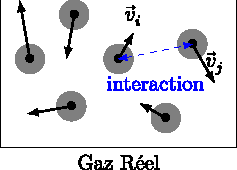
\includegraphics[width=\linewidth]{gaz_reel}
		\end{minipage}
		\begin{minipage}{0.49\linewidth}
			\centering
			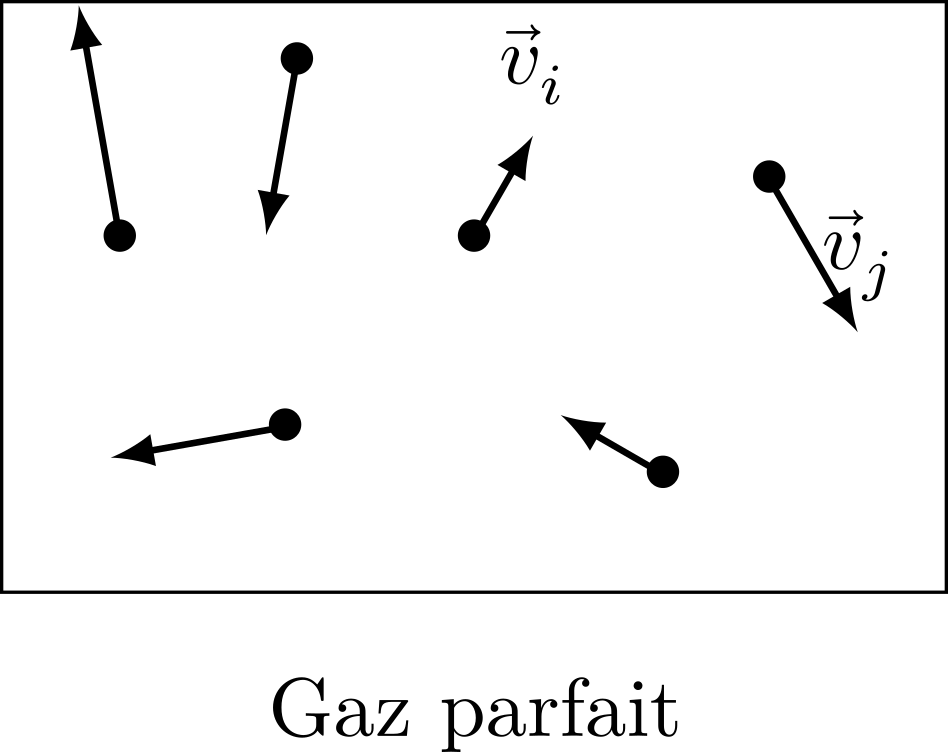
\includegraphics[width=\linewidth]{gaz_parfait}
		\end{minipage}
	\end{tcb}
	\begin{tcb}[label=loi:gp](loi)'r'{Loi du gaz parfait}
		Lorsque la pression est assez faible ($\lesssim \SI{1}{bar}$) et à des
		températures assez élevées, les grandeurs physiques décrivant un gaz
		sont reliées par la formule
		\csw{
			\begin{gather*}
				\boxed{pV = nRT}
				\qavec
				\left\{
				\begin{array}{ll}
					p & \text{en Pa }                 \\
					V & \text{en m}^3                 \\
					n & \text{en mol}                 \\
					T & \text{en \textbf{Kelvin} (K)}
				\end{array}
				\right.
			\end{gather*}
		}
		avec
		\csw{
			\begin{gather*}
				\boxed{R = \SI{8.314}{J.mol^{-1}.K^{-1}}}\\
				\text{la constante des gaz parfaits}
			\end{gather*}
		}
		\vspace{-15pt}
	\end{tcb}
\end{tcbraster}
\begin{tcb}[label=appl:gp, sidebyside](appl){Application}
	On considère une seringue cylindrique de \SI{10}{cm} le long et de
	\SI{2.5}{cm} de diamètre, contenant \SI{0.250}{g} de diazote de masse
	molaire $M({\rm N}_2) = \SI{28.01}{g.mol^{-1}}$ à la
	température $T = \SI{20}{\degreeCelsius}$.
	\begin{enumerate}
		\item Calculer le volume de la seringue
		\item Calculer la quantité de matière dans la seringue
		\item Calculer la pression exercée par le diazote dans la seringue
	\end{enumerate}
	\tcblower
	\begin{enumerate}
		\item
		      \csw{
			      $\boxed{V = \pi \frac{d^{2}}{4}\times \ell} = \xul{\SI{49}{cm^{3}}}$
		      }
		\item
		      \csw{
			      $\boxed{
					      n_{\ce{N_2}} = m_{\ce{N_2}}/M(\ce{N_2})} =
				      \xul{\SI{8.93e-3}{mol}
				      }$
		      }
		      \mitem
		      \csw{
			      \begin{gather*}
				      \boxed{p=\frac{nRT}{V}}
				      \\
				      \qav
				      \left\{
				      \begin{array}{rcl}
					      n & = & \SI{8.93e-3}{mol}
					      \\
					      R & = & \SI{8.314}{J.mol^{-1}.K^{-1}}
					      \\
					      T & = & \SI{20}{\degreeCelsius} = \SI{293.15}{K}
					      \\
					      V & = & \SI{49}{cm^{3}} = \SI{49e-6}{m^{3}}
				      \end{array}
				      \right.\\
				      \AN
				      \xul{
					      p = \SI{4.4e5}{Pa} = \SI{4.4}{bars}
				      }
			      \end{gather*}
		      }
	\end{enumerate}
\end{tcb}

\begin{tcbraster}[raster columns=2, raster equal height=rows]
	\begin{tcb}[label=def:volmol](defi){Volume molaire}
		Le \textbf{volume molaire} $V_m$ d'un corps est le volume occupé par
		\textbf{une mole} de gaz~:
		\csw{
			\[\boxed{V_m = \frac{V}{n}} \Leftrightarrow n = \frac{V}{V_m}\]
		}
		\tcbsubtitle{\fatbox{Unités}}
		\csw{
		$V_m$ s'exprime en $\si{m^3.mol^{-1}}$ ou en $\si{L.mol^{-1}}$
		}
	\end{tcb}
	\begin{tcb}[label=exem:volmol](appl)'r'{Volume molaire}
		Calculer le volume molaire d'un gaz parfait pour $\theta_1 =
			\SI{0}{\degreeCelsius}$ et $\theta_2 = \SI{25}{\degreeCelsius}$ avec $p
			= \SI{1013}{hPa}$.
		\tcblower
		\csw{
			\begin{gather*}
				T_1 = \SI{273.15}{K} \Rightarrow \DS V_m = \frac{RT}{p} =
				\SI{22.4}{L.mol^{-1}}
				\\
				T_2 = \SI{298.15}{K} \Rightarrow \DS V_m = \frac{RT}{p} =
				\SI{24.5}{L.mol^{-1}}
			\end{gather*}
		}

	\end{tcb}
\end{tcbraster}

\subsubsection{Pression partielle}
\begin{tcb}[label=def:ppartielle](defi){Pression partielle}
	La \textbf{pression partielle} $P_i$ d'une espèce gazeuse $\ce{X}_i$ au
	sein d'un mélange de \textbf{gaz parfaits} de volume $V$ et de température $T$ est
	égale à la \textbf{pression qu'aurait le système si l'espèce $\ce{X}_i$
		était la seule à occuper tout le volume}~:
	\csw{
		\[\boxed{P_iV = n_{g,i} RT}\]
	}
\end{tcb}
\begin{tcb}[width=\linewidth](appl){Exercice}
	On note $P$ la pression totale d'un mélange de gaz parfaits, et $P_i$ la
	pression partielle d'un constituant $\ce{X}_i$. Montrer que $\sum_i P_i = P$.
	\tcblower
	\csw{
		\[
			\sum_i P_i = \sum_i \frac{n_{g,i}RT}{V} = \frac{RT}{V} \sum_i n_{g,i} =
			\frac{n_{g,\tot}RT}{V} = P
			\qed
		\]
	}
\end{tcb}

\subsubsection{Loi de \textsc{Dalton}}
\begin{tcbraster}[raster columns=2, raster equal height=rows]
	\begin{tcb}[label=loi:dalton](loi){Loi de \textsc{Dalton}}
		Soit un mélange de gaz parfaits de pression $P$. Les pressions
		partielles $P_i$ de chaque constituant $\ce{X}_i$ s'exprime
		\csw{
			\[\boxed{P_i = x_iP}\]
		}
		\vspace{-15pt}
	\end{tcb}
	\begin{tcb}[label=demo:dalton](demo)'r'{Loi de \textsc{Dalton}}
		\csw{
			\[
				P_i =\frac{n_{g,i}RT}{V} = \xunderbracket{\frac{n_{g,i}}{n_{g,\tot}}}_{x_i}
				\times \xunderbracket{\frac{n_{g,\tot}RT}{V}}_{P}
				\Lra
				\boxed{P_i = x_iP}
				\qed
			\]
		}
	\end{tcb}
\end{tcbraster}

\begin{tcb}[breakable](appl){Exercice}
	Soit un mélange de gaz nobles contenu dans une enceinte de \SI{100}{L} à la
	température $T = \SI{298.3}{K}$, avec \SI{2}{mol} d'hélium He, \SI{5}{mol}
	d'argon Ar et \SI{10}{mol} de néon Ne.
	\smallbreak
	Calculer la pression totale dans l'enceinte aussi que la partielle de chacun
	des gaz.
	\smallbreak
	On donne la constante du gaz parfait $R = \SI{8.31}{J.K.mol^{-1}}$.
	\smallbreak
	Conseil~: \textbf{FAIRE UN SCHÉMA}
	\tcblower
	\begin{isd}
		\csw{
			\begin{gather*}
				n_{g,\tot} = \SI{17}{mol} \Ra P = \frac{n_{g,\tot}RT}{V}
				\\
				\qav
				\left\{
				\begin{array}{rcl}
					n_{g,\tot} & = & \SI{17}{mol}
					\\
					R          & = & \SI{8.31}{J.mol^{-1}.K^{-1}}
					\\
					T          & = & \SI{298.3}{K}
					\\
					V          & = & \SI{100}{L} = \SI{0.1}{m^{3}}
				\end{array}
				\right.\\
				\AN
				\xul{
					P = \SI{4.2e5}{Pa}
				}
				\\
			\end{gather*}
		}
		\tcblower
		\csw{
			\begin{align*}
				\Aboxed{P_{\ce{Ar}} & = \frac{n_{\ce{Ar}}}{n_{g,\tot}}P} = \xul{\SI{1.2e5}{Pa}}
				\\
				\Aboxed{P_{\ce{He}} & = \frac{n_{\ce{He}}}{n_{g,\tot}}P} = \xul{\SI{0.50e4}{Pa}}
				\\
				\Aboxed{P_{\ce{Ne}} & = \frac{n_{\ce{Ne}}}{n_{g,\tot}}P} = \xul{\SI{2.5e5}{Pa}}
			\end{align*}
		}
	\end{isd}
\end{tcb}

\subsection{Intensivité, extensivité}
\begin{tcbraster}[raster columns=2, raster equal height=rows]
	\begin{tcb}[label=def:intext](defi){Grandeurs intensives et extensives}
		\begin{itemize}
			\bitem{Intensive}~:
			\csw{
				sa valeur ne dépend pas de la taille du système~;
			}
			\bitem{Extensive}~:
			\csw{
				elle est proportionnelle à une quantité caractéristique du système.
			}
		\end{itemize}
	\end{tcb}
	\begin{tcb}[label=exem:intext](exem)'r'{Grandeurs intensives et extensives}
		\csw{
			La \textbf{pression} ou la \textbf{température} sont
			\textbf{intensives}~: deux gaz à la même température qui sont mélangés
			restent à la même température.
			\smallbreak
			La \textbf{masse} ou le \textbf{volume} sont \textbf{extensives}.
		}
	\end{tcb}
\end{tcbraster}

\subsection{Activité}
Enfin, pour suivre l'évolution d'un système qui subit une transformation
chimique, on utilise l'\textbf{activité} chimique des espèces, notée $a(\ce{X})$
pour l'espèce $\ce{X}$. Elle quantifie \textbf{l'écart des propriétés} de
l'espèce en question par rapport à un \textbf{état standard}~: on définit
\begin{itemize}
	\item \csw{
		      $c\degree = \SI{1}{mol.L^{-1}}$ la concentration standard~;
	      }
	\item \csw{
		      $P\degree = \SI{1}{bar} = \SI{e5}{Pa}$ la pression standard.
	      }
\end{itemize}

\begin{tcb}[label=ror:activité,
		tabularx*={\renewcommand{\arraystretch}{2}}{Y|Y},
		heart](ror){Activité chimique}
	\textbf{État physique}  & \textbf{Activité}\\\hline
	Gaz (pur ou mélange)    & \csw{
		$a(\ce{X\gaz{}}) = \dfrac{P_\ce{X}}{P\degree}$
	}
	\\\hline
	Liquide ou solide (PUR) & \csw{
		$a(\ce{X\liq{}}) = a(\ce{X}\sol) = 1$
	}
	\\\hline
	Soluté (assez dilué)    & \csw{
		$a(\ce{X\aqu{}}) = \dfrac{[\ce{X}]}{c\degree}$
	}
	\\\hline
	Solvant                 & \csw{
		$a_{\rm solvant} = 1$
	}
\end{tcb}

\end{document}
